\chapter{Bias\cite{nienhuys1997foundations}}\label{ch:bias}
Considering all theories $H \subseteq L$ as possible hypotheses is computationally infeasible. When one knows the properties that a hypothesis may take, one may introduce a bias $\mathcal{H} \subseteq \powerset{L}$ and then restrict a search for hypotheses $H \in \mathcal{H}$. For example, $\mathcal{H}$ being a set of all finite Horn theories.

Two main types of a bias are:
\begin{itemize}
\item language bias,
\item search bias.
\end{itemize}

ILP systems use bias to refine their search space $\mathcal{H}$, to induce a preference relation on the space of hypotheses and to control their search. The objective of this section is to classify the ILP systems based on the biases they use and the capabilities of their biases of a certain type.

First we formalise a theory of the language bias \ref{sec:background_language_bias} by using Muggleton's mode language and defining the concepts of determination language and meta-constraint language present in the implementations of ILP systems.
We establish a correspondence between this new formalism of a language bias specification and a theoretical specification of Inoue \cite{inoue1992linear} of a language bias by a production field. Then we classify ILP systems by their language bias \ref{sec:classification_language_bias} using the new formalism.
We provide a summary of algorithms for finding a hypothesis for each classified ILP system and classify ILP systems by a search bias \ref{classification_by_search_bias} arising from this search algorithm.

In the context of a language bias we refer to the bias as a hypothesis space $\mathcal{H}$, in the context of a search bias we refer to it as a search space $\mathcal{H}$.
These different terminologies refer to the same bias $\mathcal{H}$, however emphasise a different local focus on a bias in the text.

\section{Theory of language bias}\label{sec:background_language_bias}
The space of all possible hypotheses $H \in \mathcal{H}$ is restricted by a language bias $\mathcal{H}$ (called a syntactic bias in \cite{muggleton1994inductive}). The author presents the main types of the language biases in ILP:
\begin{itemize}
\item mode declarations,
\item determinations,
\item meta-constraints,
\item induction and production field.
\end{itemize}

The author concludes the section by establishing the correspondence between these known and newly formalised types of a language bias.

\subsection{Mode declarations}\label{background_mode_declarations}
Mode declarations specify what predicates are allowed in a head and a body of a hypothesis.
Suppose you would like your ILP system explain observations
$woman(alice), woman(susan)$, then you know that a hypothesis you are looking for has to explain or define the concept $woman$. Therefore you declare a statement to an ILP system: ``In your search consider only hypotheses that have the predicate $woman$ in their head." A statement specifying what predicates should be in a head is called a modeh declaration. A statement specifying the allowed predicates in a body is a modeb declaration.

\paragraph{Mode declaration in Progol}
Muggleton defines the hypothesis bias $\mathcal{H}$ with mode language and mode declarations.
\begin{defn}\cite{muggleton1995inverse}
A \emph{mode declaration} has either the form
\tc{modeh(n,atom)} or \tc{modeb(n,atom)} where $n$, the \emph{recall}, is either an integer, $n \ge 1$,
or \tc{*} and atom is a ground atom. Terms in the atom are either normal or place-marker. A normal term is either a constant or a function symbol followed by a
bracketed tuple of terms. A place-marker is either \tc{+type}, \tc{-type} or \tc{\#type}, where
type is a constant. If $m$ is a mode declaration then $a(m)$ denotes the atom of m
with place-markers replaced by distinct variables. The sign of $m$ is positive if $m$
is a \tc{modeh} and negative if $m$ is a \tc{modeb}.
\end{defn}

The recall is used to bound the number of alternative solutions for instantiating
the atom. For simplicity, we assume in the following that all the modes have the
recall \tc{*}, meaning all solutions. The following defines when a clause is within Progol's definite mode language $L$.

\begin{defn}\label{definition_definite_mode_language}\cite{muggleton1995inverse}
Let $C$ be a definite clause with a
defined total ordering over the literals and $M$ be a set of mode declarations.
$C = h \leftObjectImplies b1, ..., bn$ is in the \emph{definite mode language} $L(M)$ iff 1) $h$ is the atom
of a \tc{modeh} declaration in $M$ with every place-marker \tc{+type} and \tc{-type} replaced by
variables and every place-marker \tc{\#type} replaced by a ground term and 2) every
atom $b_i$ in the body of $C$ is the atom of a \tc{modeb} declaration in $M$ with every
place-marker \tc{+type} and \tc{-type} replaced by variables and every place-marker \tc{\#type}
replaced by a ground term and 3) every variable of \tc{+type} in any atom $b_i$ is either
of \tc{+type} in $h$ or of \tc{-type} in some atom $b_j$, $1 \le j < i$.
\end{defn}

\begin{exmp}
The mode declarations $M=\{$
\begin{lstlisting}
modeh(1,woman(+person)),
modeb(*,female(+person)),
modeb(*,male(+person))
\end{lstlisting}
$\}$
specify the possible hypotheses
$H_1=woman(X)$,
$H_2=woman(X) \leftObjectImplies female(X)$,
$H_3=woman(X) \leftObjectImplies male(X)$,
$H_4=woman(X) \leftObjectImplies female(X), male(X)$.
Therefore the hypothesis bias created by the mode declarations 
is $\mathcal{H}=L(M)=\{H_1, H_2, H_3, H_4\}$, but $H_5 \not\in L(M)$ for
$H_5=woman(X) \leftObjectImplies cook(X)$.
\end{exmp}

The mode declarations can have a richer syntactic structure where \tc{?} in the last modeb declaration stands for an arithmetical operator:
\begin{exmp}\cite{muggleton1995inverse}
\begin{lstlisting}
modeh(1,plus(+int,+int,-int))
modeb(*,append(-list,+list,+list)
modeb(1,append(+list,[+any],-list))
modeb(4,(+int ? #int))
\end{lstlisting}
\end{exmp}

\subsection{Determinations}\label{bias_determinations}
Some ILP systems like Aleph \cite{aleph2007} in addition to mode declarations use determination statements to impose a finer control on a search space.

\begin{defn}\cite{aleph2007}
A \emph{determination} is a logic statement of the form\\
\tc{determination(TargetName/TargetArity, BackgroundName/BackgroundArity).}
where \tc{TargetName}, \tc{BackgroundName} are predicate symbols and
\tc{TargetArity}, \tc{BackgroundArity} are their arities (non-negative integers) respectively.
\end{defn}

\begin{defn}\label{definition_determination_language}
Let $D=\langle d_1(tn_1/ta_1, bn_1/ba_1), ..., d_n(tn_n/ta_n, bn_n/ba_n)\ \rangle$ be an ordered list of determinations. A formula $H=h \leftObjectImplies b_1, ..., b_m$ is in \emph{determination language} $L(D)$ iff\\
1) $D \not=\emptyset$,\\
2) $\forall b_i (1 \le i \le m) \exists j (1 \le j \le n) tn_j=h \land bn_j=b_i$.
\end{defn}

\begin{exmp}
Let $D$ be the list of the determinations
\begin{lstlisting}
:− determination(man/ 1, male/1).
:− determination(man/ 1, bridegroom/1).
:− determination(woman/ 1, female/1).
\end{lstlisting}
Let the hypotheses be

\begin{minipage}[t]{.50\textwidth}
\begin{lstlisting}
H1=man(X) :- male(X).
H2=man(X) :- bridegroom(X).
H3=man(X) :- male(X), bridegroom(X).
\end{lstlisting}
\end{minipage}
\begin{minipage}[t]{.50\textwidth}
\begin{lstlisting}
H4=woman(X) :- female(X).
H5=man(X) :- male(X), female(X).
\end{lstlisting}
\end{minipage}

Then for the hypothesis bias (determination language) $\mathcal{H}=L(D)$,
$\{H_1, H_2, H_3, H_4, H_5\} \cap \mathcal{H}=\{H_1, H_2, H_3\}$.
\end{exmp}

\subsection{Meta-constraints}\label{bias_meta-constraints}
Meta-constraints specify the additional constraints on the hypothesis space $\mathcal{H}$ not definable with the mode declarations and determinations.
An example being a meta-constraint $Cond$ specifying the maximum number of the literals allowed in a formula $H \in L$.

\begin{defn}
A \emph{meta-constraint} on a language $L$ is any formula $Cond$ defining some subset $L(Cond)$ (\emph{meta-constraint language}) of the language $L$, i.e. $L(Cond)=\{x \in L | Cond(x)\}\subseteq L$.
\end{defn}

Each ILP system has its own set of allowed meta-constraints.
\begin{exmp}
In Toplog \tc{set(maximum\_literals\_in\_hypothesis, 5)} defines clausal theories whose clauses consist of at most 5 literals.
In Imparo \tc{set\_max\_clauses(2)} defines clausal theories with at most 2 clauses.
In Tal \tc{option(max\_body\_literals, 5)} defines definite theories whose clauses have at most 5 positive literals.
\end{exmp}

\begin{proposition}
Let $Cond_1, Cond_2$ be meta-constraints on a language $L$.
Then $Cond_1 \land Cond_2$ is a meta-constraint on the language $L$.
\end{proposition}

\begin{proof}
Follows trivially from the definition of a meta-constraint.
\end{proof}

Therefore we will often think of a set of the meta-constraints to be a meta-constraint created from their conjunction.

\begin{defn}
Let $C=\{Cond_1, ..., Cond_n\}$ be a set of meta-constraints defining subsets of the language $L$.
A \emph{meta-constraint language} $L(C)$ is the intersection of the subsets defined by $Cond_1, ..., Cond_n$,
i.e. $L(C)=\{x \in L | Cond_1(x) \land ... \land Cond_n(x) \}$.
\end{defn}

\begin{exmp}
Let $Cond_1$ be a meta-constraint representing all clausal theories with at most one clause. Let $Cond_2$ be a meta-constraint representing all clausal theories whose members are definite clauses. Then $L(Cond_1 \land Cond_2)$ is a language of all theories containing exactly one definite clause.
\end{exmp}

\subsection{Induction and production field}
Inoue defines a production field as another form of a language bias.

\begin{defn}\cite{inoue2004induction}
A \emph{production field} $\mathcal{P}$ is a represented by a pair,
$\langle Lit, Cond\rangle$, where $Lit$
(\emph{the characteristic literals} of $\mathcal{P}$) is a subset of literals in a language $L$ and is closed under instantiation (that is, if a literal containing variables is in $Lit$, then all its instances are also in $Lit$), and $Cond$ is a certain condition to be satisfied. 
A clause $C$ is said to \emph{belong to a production field} $\mathcal{P} = \langle Lit, Cond \rangle$ if every literal in $C$ belongs to $Lit$ and $C$ satisfies $Cond$.
\end{defn}


\begin{defn}\label{induction_field_definition}\cite{yamamoto2012inverse}
An \emph{induction field} denoted $\mathcal{I}_H=\langle Lit \rangle$ is a production field $\langle Lit, true\rangle$.
\end{defn}

\begin{defn}\cite{yamamoto2012inverse}
A ground hypothesis $H_g$ \emph{belongs to} an induction field $\mathcal{I}_H=\langle Lit \rangle$ iff
every literal in $H_g$ is included in $Lit$.
\end{defn}

\begin{exmp}
Let a set of literals be $Lit=\{p, q, r\}$ and a condition $Cond$ on a clause $C$ be $Cond(C) \iff \#C=2$, then the production field
$\langle Lit, Cond \rangle = \{ p \lor q, p \lor r, q \lor r\}$ and the induction field $\langle Lit \rangle = \langle Lit, true \rangle = \{\square, p, q, r, p \lor q, p \lor r, q \lor r, p \lor q \lor r\}$ where $\square$ is an empty clause.
Then $H=p \leftObjectImplies q \equiv p \lor \neg q$ does not belong to an induction field $\langle Lit \rangle$ or a production field $\langle Lit, Cond \rangle$, but $H$ belongs to an induction field $\langle Lit \cup \{\neg q\} \rangle$ and to a production field $\langle Lit \cup \{\neg q\}, Cond \rangle$.
\end{exmp}

\subsection{Correspondence between mode declarations, determinations, meta constraints and production field}\label{bias_correspondence}
We prove that a production field is a generalization of mode declarations, determinations and meta-constraints and hence establish a correspondence between our formalism of a language bias specification capturing the notions encountered in implementations of ILP systems and an implementation independent formalism of a language bias specification by Inoue.

\begin{proposition}\label{md_d_pf_correspondence_proposition}
Let $M$ be a set of mode declarations, $D$ an ordered list of determinations. Then there exist production fields
$\mathcal{P}_M$,
$\mathcal{P}_D$,
$\mathcal{P}_{M,D}$
such that for any clause $H \in L$:\\
1) $H \in L(M) \iff H \in \mathcal{P}_M$,\\
2) $H \in L(D) \iff H \in \mathcal{P}_D$,\\
3) $H \in L(M) \cap L(D) \iff H \in \mathcal{P}_{M,D}$.\\
\end{proposition}
The following proof is non-constructive.
\begin{proof}
Let $L$ be a logic language. By the definitions of definite mode language \ref{definition_definite_mode_language} and determination language \ref{definition_determination_language}, $L(M)$ and $L(D)$ are definable.
Let $Cond_M$, $Cond_D$ be defining formulas for $L(M)$ and $L(D)$, i.e. $L(M)=\{x \in L | Cond_M(x)\}$, $L(D)=\{x \in L | Cond_D(x)\}$.
Let $Cond_{M,D}=Cond_M \land Cond_D$. Let $Lit$ be a set of all literals of $L$ and let
$Lit_M=L(M) \cap Lit$,
$Lit_D=L(D) \cap Lit$,
$Lit_{M,D}=Lit_M \cap Lit_D$.
Then for every clause $H \in L$ the production fields
$\mathcal{P}_M=\langle Lit_M, Cond_M \rangle$,
$\mathcal{P}_D=\langle Lit_D, Cond_D \rangle$,
$\mathcal{P}_{M,D}=\langle Lit_{M,D}, Cond_{M,D} \rangle$
satisfy the conditions 1, 2, 3 respectively trivially.
\end{proof}

Given production fields defining the bias of mode declarations and determinations, we prove that productions fields with additional meta-constraints can be constructed.

\begin{proposition}\label{proposition_meta-constraints_production_field}
Let $\mathcal{P}$ be any production field, $C$ a set of meta-constraints.
Then there exists a production field $\mathcal{P}_C$ such that
$\mathcal{P}_C=\mathcal{P} \cap L(C)$, i.e.
$\forall H \in L. H \in \mathcal{P}_C \iff (H \in \mathcal{P}) \land (H \in L(C))$.
\end{proposition}
\begin{proof}
Let $\mathcal{P}=\langle Lit, Cond \rangle$,
$C=\{Cond_1, ..., Cond_n\}$.
Define $\mathcal{P}_C=\langle Lit, Cond \land Cond_1 \land ... \land Cond_n \rangle$. Take an arbitrary $H \in L$. Denote $Lit(H)$ to be the set of the literals of the clausal form of $H$.
Then $H \in \mathcal{P}_C$ iff $Lit(H) \subseteq Lit$ and
$(Cond \land Cond_1 \land ... \land Cond_n)(H)$ iff
$Lit(H) \subseteq Lit$ and $Cond(H)$ and $Cond_1(H) \land ... \land Cond_n(H)$
iff $H \in \langle Lit, Cond \rangle = \mathcal{P}$ and $H \in L(Cond_1 \land ... \land Cond_n) = L(C)$. Thus $\mathcal{P}_C=\mathcal{P} \cap L(C)$.
\end{proof}

\begin{corollary}
Let $M$ be a set of mode declarations, $D$ an ordered list of determinations, $C$ a set of the meta-constraints.
Then there exist production fields
$\mathcal{P}_{M,C}$,
$\mathcal{P}_{M,D,C}$
such that for any clause $H \in L$:\\
1) $H \in L(M) \cap L(C) \iff H \in \mathcal{P}_{M,C}$,\\
2) $H \in L(M) \cap L(D) \cap L(C) \iff H \in \mathcal{P}_{M,D,C}$.\\
\end{corollary}
\begin{proof}
Follows from \ref{md_d_pf_correspondence_proposition} and \ref{proposition_meta-constraints_production_field}.
\end{proof}

The converse depends on the possible meta-constraints. If one allowed a meta-constraint for every possible definable condition $Cond$, then one could express any production field $\mathcal{P}=\langle Lit, Cond \rangle$ with mode declarations, determinations and meta-constraints.

\section{Classification by language bias}\label{sec:classification_language_bias}
In this subsection we use our formalism of a language bias specification to 
classify ILP systems based on their peculiarities related to the language bias: mode declarations, determinations and meta-constraints.

\subsection{Mode declarations}\label{classification_mode_declarations}
We summarise the use of mode declarations in an ILP system and their defining role.

We examine the compatibility of mode declarations with the mode declarations of Progol since mode declarations were first defined for Progol in seminal work by Muggleton\cite{muggleton1995inverse}.
We say that a system of mode declarations is \emph{Progol compatible} iff any hypothesis bias definable with Progol mode declarations can be defined within that system.

\begin{center}
\captionof{table}{Classification by mode declaration bias} \label{tab:classification_by_mode_declaration_bias} 
 \begin{tabular}{| l | l | l | l | l | l | l |}
    \hline
    Mode declarations/ILP system & Progol & Aleph & Toplog & Xhail & Imparo & Tal \\ \hline
    Progol compatible & yes & yes & no &  yes & no & no \\ \hline
    Recall modeb support & yes & yes & yes & yes & no & yes \\ \hline
    Recall modeh support & yes & yes & no & yes & no & no \\ \hline
    Recall lower bound support & no & no & no & yes & no & no \\ \hline
  \end{tabular}
  \end{center}

We further support the statements in a summary by examining a system of mode declarations for each ILP system.

\paragraph{Progol}
Progol supports the mode declarations as defined in \fullref{background_mode_declarations}.

\begin{exmp}\cite{muggleton1999progolWebsite}
\begin{lstlisting}
:- modeh(1,class(+animal,#class))?
:- modeb(1,has_gills(+animal))?
:- modeb(*,habitat(+animal,#habitat))?
:- modeh(1,append([+constant|+clist],+clist,[-constant|-clist]))?
:- modeh(1,append(+clist,+clist,-clist))?
\end{lstlisting}
\end{exmp}

\paragraph{Aleph}
Aleph's mode declarations are compatible\cite{aleph2007} with the mode declarations specified by Progol.
\begin{exmp}
\begin{lstlisting}

:-modeh(1, woman(+person)).
:-modeb(1, female(+person)).
:-modeb(*, english_couple(+person, -person)).
:-modeb(2, english(+person)).
\end{lstlisting}
\end{exmp}

\paragraph{Toplog}
Toplog's modeb declarations are compatible with Progol up to specification of the atom. Specification of the recall is optional, however, for modeh declarations recall cannot be specified\cite{santos2008toplogWebsite}.
\begin{exmp}\cite{santos2008toplogWebsite}
\begin{lstlisting}
:-modeh(append(+list,+list,-list)).
:-modeb(append(+list,+list,-list)).
:-modeb(5,append(+list,+list,-list)).
:-modeh(class(+animal,#class)).
:-modeh(*,uncle(+person, -person)).%invalid
\end{lstlisting}
\end{exmp}

\paragraph{Xhail}\label{xhail_mode_declarations}
Xhail has extended mode declarations to include meta-constraint statements in order to refine its search space.

Xhail executable's help\cite{ray2007xhail} reads:
\begin{quote}
\emph{Zero or more head declarations} are of the form
\tc{modeh(1,3,min,p("\#q","+r","-s"))} meaning between 1 and 3 ground atoms
 of the form $p(a,b,c)$ should be assumed such that $q(a), r(b), s(c)$ hold 
 and where $a, b, c$ are constant, input, output terms, respectively;
 the third flag is either min="attempt to minimize" or all="do not minimize".
 
\emph{Zero or more body declarations} are of the form \tc{modeb(1,3,pos,p("\#q","+r","-s")).} meaning this scheme can be used between 
 depths 1 and 3.  The third flag is either pos="pos. literal" or neg="neg. literal" 
\end{quote}

\begin{exmp}\ref{xhail_fine_search_space_control}
\begin{lstlisting}
modeh(0,1,all,woman("+person")).
modeb(0,1,pos,female("+person")).
\end{lstlisting}
\end{exmp}

Whereas Progol specifies the recall by its upper bound, Xhail enables its specification for both its \emph{lower bound} and upper bound. meta-constraint statements
\tc{min}, \tc{all}, \tc{pos}, \tc{neg} constraint the hypothesis bias further.

\paragraph{Imparo}\cite{kimber2013imparo}
Imparo does not support recall specification in its mode declarations. The specification of the atom is supported.
\begin{exmp}
\begin{lstlisting}
head_modes([
    woman(+number)
]).
body_modes([
    female(+number)
]).
\end{lstlisting}
\end{exmp}

\paragraph{Tal}
Tal does not support recall specification for modeh declarations, however the recall can be specified for the modeb declarations\cite{corapi2011tal}.
\begin{exmp}
\begin{lstlisting}
modeh(happens("#event","#time","#scenario")).
modeh(woman(+person), [name(wh)]).
modeb(female(+person), [name(fb)]).
modeb(2,female(+person), [name(fb)]).
\end{lstlisting}
\end{exmp}

\subsection{Determinations}\label{classification_determinations}
By reading the manuals of the corresponding ILP systems, one may find that
Toplog, Xhail, Imparo, Tal do not support the determinations.
Progol supports the use of the determinations, cf. \ref{progol_multiclausal_learning}, but it does not require it, cf. \ref{progol_specialization_in_arguments}.
Aleph requires the determinations to be specified as in \ref{subsec:aleph_determination_declaration_requirement}.

\subsection{Meta-constraints}\label{classification_meta-constraints}
Meta-constraints supplement mode declarations and determinations in specifying a language bias. We select several meta-constraints and evaluate their support  across the ILP systems classified:

\begin{itemize}
\item the maximum number of literals in a clause of a hypothesis,
\item the maximum number of clauses in a hypothesis - some incomplete ILP systems do not support multiclausal hypotheses, therefore they do not need and cannot support this meta-constraint,
\item the maximum variable depth (definition \ref{definition_variable_depth}) of a hypothesis,
\item the (minimum and maximum) number of singletons in a hypothesis:
a singleton is a variable that appears only once in a hypothesis\cite{santos2008toplogWebsite}
\end{itemize}

The support for the meta-constraints of interest is summarised first, the claims are supported afterwards.

\begin{center}
\captionof{table}{Classification by meta-constraints} \label{tab:classification_by_meta-constraints} 
 \begin{tabular}{| l | l | l | l | l | l | l |}
    \hline
    meta-constraint/ILP system & Progol & Aleph & Toplog & Xhail & Imparo & Tal \\ \hline
    Max. no. of literals in a clause & no & yes & yes & no & yes & yes\\ \hline
    Max. no. of clauses in $H$ & no & yes & no & no & yes & yes\\ \hline
    Max. variable depth in $H$ & no & yes & no & no & yes & no\\ \hline
    Number of singletons in $H$ & no & no & yes & no & no & no\\ \hline
  \end{tabular}
  \end{center}
  
If one considered the chosen meta-constraints as representative, then it could be deduced that Progol and Xhail have the most trivial system of specifying a language bias with meta-constraints whereas Aleph and Imparo have the most powerful system.

\paragraph{Variable depth}
\begin{defn}\label{definition_variable_depth}\cite{nienhuys1997foundations}
The \emph{variable depth of a variable} $x$ in an ordered definite program clause
$A \leftObjectImplies  B_1, . . . , B_n$ is defined as follows. If $x$ occurs in $A$, then its variable depth is $0$. Suppose $x$ first occurs in $B_i$.
If none of the other variables
in $B_i$ already occurred in $A \leftObjectImplies B_1,... ,B_{i-1}$,
then $x$ has variable depth $\infty$.
Otherwise, the variable depth of $x$ is $1$ plus the variable depth of the variable in $B_i$ with greatest variable depth occurring in
$A \leftObjectImplies B_1,... ,B_{i-1}$.
The \emph{variable-depth of a clause} in an ordered definite program
is the largest variable depth of its variables. Note that such a
clause is constrained iff it has variable depth $0$.
\end{defn}

\begin{exmp}
Let $H=path(X,Y) \leftObjectImplies path(X,X_1), arc(X_1,X_2), path(X_2,Y)$.
Then the variable depths of the variables $X,Y,X_1,X_2$ in $H$ are
$0,0,1,2$ respectively.
\end{exmp}

\paragraph{Progol}
Progol can learn only single-clausal hypotheses\cite{muggleton2012mc}, therefore it does not support a meta-constraint specifying the number of clauses in a hypothesis.
Progol manual does not provide information about its meta-level constraints. The meta-level constraints used in the provided files\cite{muggleton1999progolWebsite} were of the following format:
\begin{lstlisting}
./pole.pl::- op(10, xfx, ...)?
./pole.pl::- op(30,xfy,:)?
./numbers.pl::- set(h,100)?
./numbers.pl::- set(r,1000)?
./numbers.pl::- set(inflate,99)?
./numbers.pl::- set(nodes,100)?
./numbers.pl::- set(i,5), set(c,5)?
\end{lstlisting}
For examining the maximum number of literals in a clause of a hypothesis meta-constraint we gave Progol a learning program where a target hypothesis had $n$ literals. Progol learnt such a hypothesis. Then we changed the parameters in the meta-constraints listed above to multiple values ($n+1$, $n$, $n-1$, $n-2$, $1$, $-1$, $-n$ and others). Progol still learnt the target hypothesis and therefore did not reduce the hypothesis space by hypotheses specified by the number of literals in their clauses. Thefore we conclude that Progol does not support this meta-constraint assuming that there are no other meta-constraints apart from those found in provided files and that numbers in a specification of metaconstraints are humanly intuitive, e.g. that a theory with at most $3$ literals in its clauses is not represented by some meta-constraint of the form \tc{:- set(i, 78234)} where a relation between numbers $3$ and $78234$ is not intuitive.

Based on the negative results of similar experiments the author assumes that Progol does not support any of the meta-constraints.

\paragraph{Aleph}
Aleph supports the first 3 chosen meta-constraints as can be consulted in the section 18 of the Aleph manual\cite{aleph2007}.
\begin{quote}
\begin{itemize}
\item (Maximum number of literals in a clause) \tc{set(clauselength,+V)}:
$V$ is a positive integer (default $4$). Sets upper bound on number of literals in an acceptable clause.
\item (Maximum number of clauses in a hypothesis) \tc{set(clauses,+V)}:
$V$ is a positive integer. Sets upper bound on the number of clauses in a theory  when performing theory-level search.
\item (Variable depth) \tc{set(i,+V)}: $V$ is a positive integer (default $2$). Set upper bound on layers of new variables.
\end{itemize}
\end{quote}

The extensive manual does not provide the information on specifying the number of singletons in a clause, hence it is assumed that this feature is not supported.

\paragraph{Toplog}
Toplog can learn only single-clausal hypotheses\cite{muggleton2012mc}, therefore it does not support a meta-constraint specifying the number of clauses in a hypothesis. It supports the specification of the maximum number $N$ of literals in a hypothesis with a meta-level statement\\
\tc{:-set(maximum\_literals\_in\_hypothesis,N)} found for example in carcinogenesis.pl file\cite{santos2008toplogWebsite}. The manual does not provide any information on the variable depth, therefore it is assumed that this feature is not supported in Toplog.
By the manual Toplog supports the specification of a maximum and minimum number of singletons in a hypothesis as can be also found in carcinogenesis.pl file:
\begin{lstlisting}
:-set(maximum_singletons_in_hypothesis,3)%carcinogenesis.pl
:-set(maximum_literals_in_hypothesis,4).%carcinogenesis.pl
\end{lstlisting}

\paragraph{Xhail}
In \ref{xhail_mode_declarations} we found out that Xhail has the most advanced system of mode declarations. On the other hand it does not support any of the chosen meta-constraints\cite{ray2007xhail}. The author consulted the Xhail's help and example files provided with Xhail as there was no access to the source code.

\paragraph{Imparo}
In a grammar learning file available with Imparo\cite{kimber2013imparo} one can find the setting:
\begin{lstlisting}
:-set_max_clause_length(6).
:-set_max_clauses(1).
:-set_max_var_depth(4).
\end{lstlisting}
Therefore Imparo supports the specification of the clausal length, the maximum number of clauses in a hypothesis and the maximum variable depth of a clause in a hypothesis (as we verified in experiments). Imparo's manual and source code do not provide any information on bounding the number of singleton variables in a clause, hence it is assumed this feature is not supported.

\paragraph{Tal}
Tal enables the specification of the clausal length by specifying the number of the literals in the body of a clause \tc{option(max\_body\_literals, N)}\cite{corapi2010inductive}. Tal specifies the number of clauses in a hypothesis with \tc{option(max\_num\_rules, N)}\cite{corapi2010inductive}, where a rule is understood as a clause. Tal's manual and source files do not mention variable depth and bounding the number of singleton variables in a clause, hence it is assumed that these features are not supported.

\section{Classification by search bias}\label{classification_by_search_bias}
Search bias\cite{nienhuys1997foundations} is defined by the properties of an algorithm that searches a hypothesis: heuristics and direction of a search. We present a hypothesis search algorithm for each ILP system and then 
we compare how ILP systems search the hypothesis space based on the search direction.
\subsection{Algorithms}

\subsubsection{Progol\cite{muggleton1995inverse}\cite{kimber2012learning}}
Progol's algorithm consists of steps:
\begin{itemize}
\item initialize $H$ to be an empty theory,
\item step 2: if $E=\emptyset$ then return $H$,
\item select an example $e \in E$,
\item construct a most specific clause within the mode language which entails $e$,
\item specialise the $\bot$ clause searching down the lattice using the A*-heuristics until a clause $h$ explaining $e$ is found, then add $h$ to $H$,
\item use the cover loop algorithm to remove all the examples from $E$ that are already explained by $H$ so far and go to step 2.
\end{itemize}

\subsubsection{Aleph}
In the Aleph manual\cite{aleph2007} a reader would find the description of the basic algorithm:
\begin{enumerate}
\item \emph{Select example.} Select an example to be generalised. If none exist, stop, otherwise proceed to the next step.
\item \emph{Build most-specific-clause.} Construct the most specific clause that entails the example selected, and is within language restrictions provided. This is usually a definite clause with many literals, and is called the "bottom clause." This step is sometimes called the "saturation" step. Details of constructing the bottom clause can be found in Stephen Muggleton's 1995 paper: Inverse Entailment and Progol\cite{muggleton1995inverse}.
\item \emph{Search.} Find a clause more general than the bottom clause. This is done by searching for some subset of the literals in the bottom clause that has the "best" score. Two points should be noted. First, confining the search to subsets of the bottom clause does not produce all the clauses more general than it, but is good enough for this thumbnail sketch. Second, the exact nature of the score of a clause is not really important here. This step is sometimes called the "reduction" step.
\item \emph{Remove redundant.} The clause with the best score is added to the current theory, and all examples made redundant are removed. This step is sometimes called the "cover removal" step. Note here that the best clause may make clauses other than the examples redundant. Again, this is ignored here. Return to Step 1.
\end{enumerate}

\subsubsection{Toplog\cite{muggleton2008toplog}\cite{corapi2011nonmonotonic}}
The Toplog algorithm used to find a hypothesis $H$ uses an extended inverse entailment following the steps:

\begin{itemize}
\item construct the \emph{top theory} $\top$ (a bias, definition \ref{definition_top_theory_bias}),
\item for every example $e \in E$:
\item derive a clause $h_e$ such that $\top \models h_e$, $B \cup \{h_e\} \models e$, add $h_e$ to $H_c$,
\item end loop,
\item select $H \in H_c$ such that $s(H)$ is maximized for a score function $s:\mathcal{H} \to \mathbb{R}$.
\end{itemize}
The score function can be based on compression, coverage, accuracy, etc.

\paragraph{Top theory\cite{muggleton2008toplog}}\label{top_theory}
In general, a \emph{top theory} is any logic theory specified on the input to an ILP system by the user, it makes sense to reason about such a logic theory wrt some hypothesis.
\begin{defn}\label{definition_top_theory_bias}
A hypothesis $H$ is in a \emph{top theory bias} wrt a top theory $\top$ iff $H \models \top$.
\end{defn}
A top theory $\top$ is a generalization of mode declarations:
\begin{exmp}(Adapted from \cite{muggleton2008toplog}.)
From the mode declarations $M$
\begin{lstlisting}
modeh(mammal(+animal)).
modeb(has_milk(+animal)).
modeb(has_eggs(+animal)).
\end{lstlisting}
a correspondent constructed top theory $\top$ is a set of clauses
\begin{lstlisting}
mammal(X) :- $body(X).
: $body(X) :- .%emptybody
: $body(X) :- has_milk(X),$body(X).
: $body(X) :- has_eggs(X),$body(X).
\end{lstlisting}
where \tc{mammal, \$body, has\_milk, had\_eggs} are their predicate symbols.
The first three clauses imply a clause $H=mammal(X) \leftObjectImplies has\_milk(X)$ (i.e. $\top \models H$)
which is indeed in mode language $L(M)$ specified by the 3 mode declarations.
\end{exmp}

\subsubsection{Xhail\cite{kimber2012learning}\cite{ray2005phdHybrid}\cite{corapi2011nonmonotonic}}
Xhail's extends the Hail's algorithm for $H$, $B$ to be normal theories following the steps:
\begin{itemize}
\item find an abductive explanation $\Delta=\{\alpha_1, ..., \alpha_n\}$ for atoms in $E$ from $B$, i.e. $B \cup \Delta \models E$,
\item find the set of atoms $\beta=\{\delta | B \models \delta\}$ that can be deduced from $B$ using SLD resolution,
\item construct a kernel set $K$ of all possible clauses with $\alpha_j \in \Delta$ in their head, and body $\{\delta^j_1, ..., \delta^j_{m_j}\} \subseteq \beta$ where any $\delta^j_i$ has to satisfy $B \cup \Delta \models \delta^j_i$,
\item find $H$ subsuming the kernel set $K$ by deleting the body literals of the clauses in $K$.
\end{itemize}

\subsubsection{Imparo}
Imparo is an ILP system based on a general IoF theoretical framework with the following algorithm:
\begin{itemize}
\item initialize $i=1$, $B_1=B$, $E^+_1=E^+$,
\item step 2: if $E^+_i = \emptyset$ then return $H=\{h_1, ..., h_{i-1}\}$,
\item select an example $e$ from the set of positive examples $E^+_i$,
\item compute the most specific connected theory (a complement of Imparo's bridge formula) for an example $e$ and the background knowledge $B_i$,
\item search the lattice of sets of clauses subsuming the connected theory and choose the hypothesis $h_i$ with the highest score according to the score function such that $B_i \cup \{h_i\} \models e$,
\item let $B_{i+1}=B_i \cup \{h_i\}$,
\item let $E^+_{i+1}=\{e' \in E^+_i | B_{i+1} \not\models e'\}$,
\item $i=i+1$, go to step 2.
\end{itemize}

\paragraph{Induction on Failure framework\cite{kimber2012learning}}
Induction on Failure framework (IoF) is a method for deriving a hypothesis $H$ where a single clause $h \in H$ does not necessarily need to explain an example $e \in E$, but an example can be explained by multiple clauses. Such a search space is called a connected theory.
\begin{defn}
A connected theory $T$ for a ground Horn clause $e$ and a Horn theory $B$ is a set of clauses that can be partitioned into sets $T_1, ..., T_n$ so that\\
(i) $B \union T_1^+ \models e_{head}$,\\
(ii) $\forall i \in \{1, ..., n-1\}. B \union e_{body} \union T_{i+1}^+ \models T_i^-$,\\
(iii) $B \union e_{body} \models T_n^-$,\\
(iv) $B \union T \not\models \square$.
\end{defn}

\subsubsection{Tal\cite{corapi2011nonmonotonic}}
Tal's algorithm is based on the use of a top theory $\top$ as Toplog combining the abductive procedure following the steps:
\begin{itemize}
\item given examples $E$, background theory $B$, mode declarations $M$, integrity constrains $I$,
\item construct a top theory $\top_M$ from $B$, $E$, $M$,
\item produce a set $\Delta$ of abductive explanations for $E$ from $\top_M \cup B$ subject to $I$,
\item derive $H$ from $\Delta$ and $M$ such that $H$ is in $L(M)$.
\end{itemize}

\subsection{Search direction\cite{nienhuys1997foundations}}
When searching for a correct hypothesis \ref{correct_hypothesis}, one may either start with an overly general hypothesis $H$ wrt $B, E^+$, $E^-$ and then try to weaken it to make it consistent with the negative examples $E^-$ while preserving its completeness wrt positive examples $E^+$. This is called a \emph{top-down} search.
On the other hand, in a \emph{bottom-up} search one starts with an overly specific hypothesis $H$ wrt $B$, $E^+$, $E^-$ and then tries to strengthen it to make it complete wrt positive examples $E^+$ while preserving the consistency wrt to the negative examples $E^-$.
The combination of both search strategies results in a \emph{mixed} search.

\begin{remark}
A reader should be careful. In the contemporary literature there are other notions and respective classes of bottom-up and top-down systems (c.f.\cite{corapi2010inductive} for Toplog). We follow the classification by Nienhuys-Cheng and Wolf\cite{nienhuys1997foundations}.
\end{remark}

We classify ILP systems based on their direction of search.

\begin{center}
\captionof{table}{Classification by hypothesis search direction}\label{tab:title} 
\begin{tabular}{| l | l | l | l | l | l | l |}
    \hline
    ILP system & Progol & Aleph & Toplog & Xhail & Imparo & Tal \\ \hline
   	Search direction & top-down & bottom-up& mixed & bottom-up & mixed & top-down\\ \hline
\end{tabular}
\end{center}

\begin{center}
\captionof{figure}{Top-down and bottom-up direction of hypothesis search}
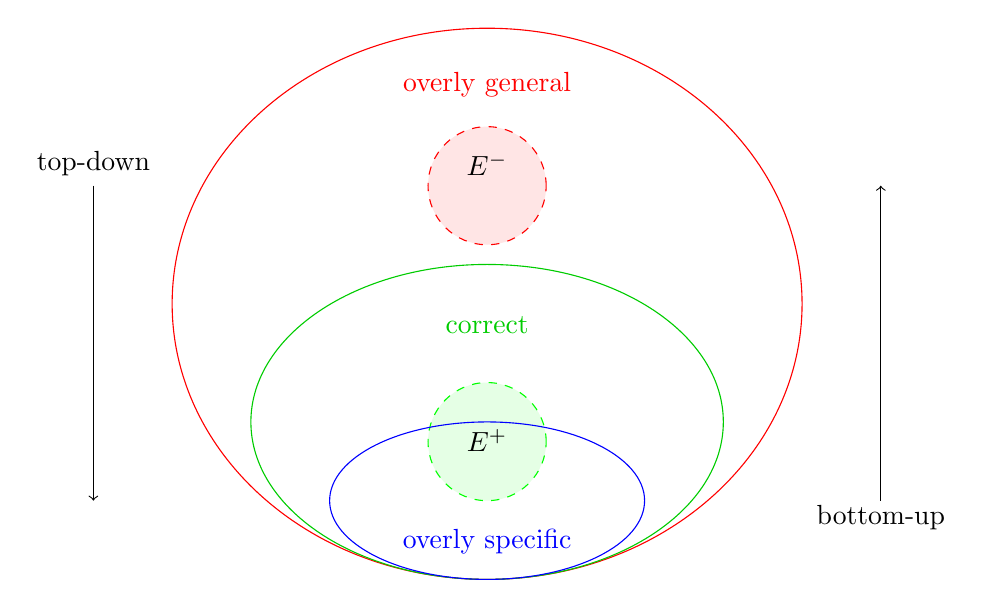
\begin{tikzpicture}
\draw[color=green, style=dashed, fill=green!10] (7, 1.75) circle (0.75);
\draw[color=red, style=dashed, fill=red!10] (7, 5) circle (0.75);
\draw[color=red] (7,3.5) ellipse (4 and 3.5);
\draw[color=green!80!black] (7,2) ellipse (3 and 2);
\draw[color=blue] (7,1) ellipse (2 and 1);
\fill (7,1.5) node[above] {$E^+$};
\fill (7,5) node[above] {$E^-$};
\fill[color=red] (7,6) node[above] {overly general};
\fill[color=green!80!black] (7,3) node[above] {correct};
\fill[color=blue] (7,0.2) node[above] {overly specific};
\draw [->] (12,1) -- (12,5);
\draw [->] (2,5) -- (2,1);
\fill (2,5) node[above] {top-down};
\fill (12,0.5) node[above] {bottom-up};
\end{tikzpicture}
\end{center}

\paragraph{Progol}
Progol searches top-down for hypotheses that subsume some bottom clause.\cite{nienhuys1997foundations}.
\paragraph{Aleph\cite{aleph2007}}
Although Aleph being based on Progol, it searches a hypothesis bottom-up. It first selects an example to be generalized, finds a bottom clause that entails it, then it generalizes the bottom clause further until a correct hypothesis is found.
\paragraph{Toplog\cite{muggleton2008toplog}}
Corapi\cite{corapi2011nonmonotonic} surveys that Toplog derives all the hypotheses $H_e$ that are generalizations of some positive example $e \in E^+$ constructing a set $H_c=\{h_e:e \in E^+\}$.
Afterwards a subset $H \in H_c$ maximizing a score function is chosen. Strictly in this sense Toplog does not perform a search. The first step of generalization is analogous to a bottom-up search. Based on the score function the second step of selection may eliminate overly general hypotheses and is therefore analogous to a top-down search. We conclude that Toplog uses a mixed hypothesis search strategy.
\paragraph{Xhail\cite{ray2003hybrid}}
Xhail (based on Hail) constructs a kernel set from the background knowledge $B$ and an example $e$ which is subsequently generalized until a correct hypothesis is found. Therefore Xhail searches a hypothesis $H$ bottom-up.

\paragraph{Imparo}
Imparo is based on the induction on failure (IoF) framework:
\begin{quote}\cite{kimber2012learning}
The procedure[IoF] interleaves top-down subsumption-based search with bottom-up generalisation of the ground connected theory T .
\end{quote}
Therefore Imparo uses a mixed strategy to search for a hypothesis.
\paragraph{Tal}
We conclude that Tal searches a hypothesis top-down from the quote bellow:
\begin{quote}\cite{corapi2010inductive}
Tal explores candidate solutions in a top-down manner,
backtracking whenever the current solution leads to failure in the abductive derivation.
\end{quote}
